\documentclass[10pt, aspectratio=169]{beamer}

% TEMA E IDENTIDADE VISUAL 
\usetheme{Madrid} 
\useoutertheme{miniframes} 
\usecolortheme{whale} 

\setbeamertemplate{blocks}[rounded][shadow=true]

\setbeamercolor{block title example}{bg=green!60!black, fg=white}
\setbeamercolor{block body example}{bg=green!10, fg=black}

%pacotes
\usepackage[utf8]{inputenc}
\usepackage[portuguese]{babel}
\usepackage{graphicx}
\usepackage{booktabs}

% capa

% o texto entre colchetes [] é o que aparece no rodapé de todos os slides
\title[Redes de Sensores Sem Fio]{Redes de Sensores Sem Fio}
\subtitle{Fundamentos, Segurança e o Futuro com Edge AI}
\author[Serafim \& Oliveira]{Waldemar Serafim Neto \and Nicolas Henrique Lima de Oliveira}
\institute[UEL]{Universidade Estadual de Londrina}
\date{2026}


\setbeamertemplate{navigation symbols}{}

\begin{document}

% slide 1: Capa
\begin{frame}
    \titlepage
\end{frame}

% slide 2: Sumário
\begin{frame}{Sumário}
    \tableofcontents
\end{frame}

% ==========================================

% estrutura inputs
% ==========================================
% quando fizer as secoes, apga o % pra descomentar

% \section{Introdução}

\begin{frame}{Contexto e Definição das RSSF}
    \begin{columns}
        \begin{column}{0.65\textwidth}
            \begin{itemize}
                \item Com o avanço da microeletrônica, os sistemas tradicionais cabeados e via satélite estão sendo substituídos por soluções mais ágeis e distribuídas.   
                \item As Redes de Sensores Sem Fio (RSSF) utilizam nós minúsculos e autônomos para monitorar grandezas específicas, como temperatura e luminosidade, em áreas de difícil acesso.   
                \item A principal vantagem dessa tecnologia é a escalabilidade, permitindo que centenas ou milhares de dispositivos formem malhas de sensoriamento de baixo custo em cidades inteligentes e indústrias.   
            \end{itemize}
        \end{column}
        
        \begin{column}{0.35\textwidth}
            \begin{figure}
                \centering
                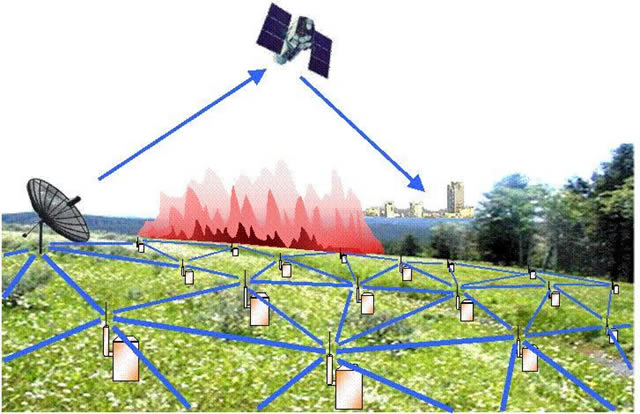
\includegraphics[width=\textwidth]{figuras/rede.jpg}
                \caption{Representação de uma RSSF.}
                \vspace{0.1cm}
                {\footnotesize Fonte: Pplware (sapo.pt)}
            \end{figure}
        \end{column}
    \end{columns}
\end{frame}

\begin{frame}{Desafios Energéticos e Resiliência}
    \begin{itemize}
        \item A operação em ambientes hostis gera restrições significativas, exigindo que os nós sensores otimizem seus escassos recursos energéticos através do processamento local de dados.   
        \item Em situações de falha (como esgotamento de bateria ou dano físico a um dispositivo), a rede precisa se reorganizar dinamicamente para garantir que o fluxo de informações não seja interrompido.   
        \item Para aumentar a sobrevida, a malha atua como um organismo reativo: os sensores permanecem em dormência profunda e despertam apenas para eventos ou alertas específicos.   
    \end{itemize}
\end{frame}

\begin{frame}{Indústria 4.0 e Objetivos do Trabalho}
    \begin{itemize}
        \item No cenário da Indústria 4.0, a conectividade distribuída dessas redes elimina cabeamentos complexos e viabiliza sistemas avançados de manutenção preditiva no chão de fábrica.   
    \end{itemize}
    
    \vspace{0.5cm}
    
    \begin{block}{Objetivo da Pesquisa}
        Apresentar os fundamentos das RSSF, detalhando suas aplicações práticas, os desafios operacionais das camadas físicas, as diretrizes de segurança cibernética e a evolução da infraestrutura com o uso da Inteligência Artificial.   
    \end{block}
\end{frame}
% \section{Visão Geral e Aplicações}

% ==========================================
% minha parte (nicola)
% ==========================================

\begin{frame}{Contexto Histórico}
    \begin{itemize}
        \item O conceito de sensoriamento distribuído surgiu na Guerra Fria com o projeto SOSUS dos EUA, focado na detecção de submarinos soviéticos. %[cite: 1]
        \item Na década de 1980, os programas da DARPA trouxeram os primeiros avanços em direção à computação distribuída moderna. %[cite: 1]
        \item A transição para uso civil ocorreu em 2004 com o surgimento de hardwares específicos (MicaZ, TelosB) e sistemas dedicados como o TinyOS. %[cite: 1]
        \item O experimento na Duck Island (2002) foi um marco prático, utilizando 150 nós para monitorar o clima e o comportamento de pássaros via satélite. %[cite: 1]
    \end{itemize}
\end{frame}

\begin{frame}{Conceitos Fundamentais: A Natureza Ad Hoc}
    \begin{itemize}
        \item As RSSF derivam das redes \textit{Ad Hoc}, formando conexões dinâmicas sem depender de infraestruturas fixas (como roteadores tradicionais). %[cite: 1]
        \item Diferente do modelo ponto-a-ponto, as RSSF focam nos dados coletados, sendo o conteúdo mais importante do que a identidade (ID) do nó que o gerou. %[cite: 1]
        \item Operam em uma topologia altamente dinâmica: a alta taxa de exaustão de baterias exige algoritmos constantes de autoconfiguração. %[cite: 1]
        \item Diferente do Wi-Fi, que foca em alta vazão, as RSSF priorizam a sobrevivência energética e o tráfego convergente para o \textit{sink node} (estação base). %[cite: 1]
    \end{itemize}
\end{frame}

\begin{frame}{Arquitetura de um Nó Sensor (Mote)}
    \begin{columns}
        \begin{column}{0.55\textwidth}
            \begin{itemize}
                \item \textbf{Subsistema de Sensoriamento:} Responsável por converter grandezas físicas (luz, temperatura, aceleração) em sinais digitais via conversores ADC.
                \item \textbf{Subsistema de Processamento:} Unidade central que gerencia o programa e armazena dados em memórias Flash e RAM.
                \item \textbf{Subsistema de Comunicação:} Interface de rádio que utiliza protocolos seriais (como SPI) para trocar informações com o processador.
                \item \textbf{Eficiência Energética:} O processamento local reduz a carga sobre o rádio, que é o componente de maior consumo[cite: 1].
            \end{itemize}
        \end{column}
        
        \begin{column}{0.45\textwidth}
            \begin{figure}
                \centering
                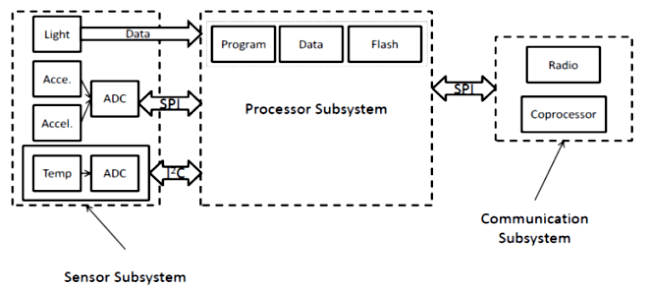
\includegraphics[width=\textwidth]{figuras/arquitetura.png}
                \caption{Arquitetura modular de um nó sensor.}
                \vspace{0.1cm}
                {\tiny Fonte: ResearchGate (Adaptado de Silva et al.)}
            \end{figure}
        \end{column}
    \end{columns}
\end{frame}

% ==========================================
% parte waldemar
% ==========================================


% \section{Camada Física e Enlace}

\begin{frame}{A Camada Física e os Padrões de Rádio}
    \begin{itemize}
        \item A Camada Física (PHY) define as especificações elétricas do meio, convertendo dados binários em sinais de Rádio Frequência (RF) ou ópticos.   
        \item A escolha pela RF é predominante por ser omnidirecional, dispensando o alinhamento geométrico rigoroso exigido por lasers.   
        \item \textbf{  Padrão IEEE 802.15.4:} Desenvolvido para mitigar instabilidades e priorizar a sobrevivência da rede, operando na frequência de 2.4 GHz com taxas de 250 kbps.   
        \item Diferente do Wi-Fi (que chega a consumir 400 mA), dispositivos 802.15.4 como o MicaZ operam com correntes baixíssimas (17 a 30 mA) e repouso profundo.   
    \end{itemize}
\end{frame}

\begin{frame}{Comunicação Óptica e o Projeto Smart Dust}
    \begin{itemize}
        \item Em projetos de miniaturização extrema, a camada física óptica ganha destaque.   
        \item O projeto \textit{Smart Dust} atinge volumes de 1 $mm^3$, utilizando modulação de feixes de luz ou espelhos reflexivos passivos.   
    \end{itemize}
    
    \vspace{0.4cm}
    
    \begin{columns}
        % --- VANTAGENS ---
        \begin{column}{0.48\textwidth}
            \begin{block}{Vantagens do Óptico}
                Altíssimas taxas de transmissão (até 1 Mbps), alcance de 10 a 100 km e consumo energético drasticamente menor que o rádio.   
            \end{block}
        \end{column}
        
        % --- DESVANTAGENS ---
        \begin{column}{0.48\textwidth}
            \begin{alertblock}{Desafios da Implementação}
                Alta vulnerabilidade a fatores climáticos e exigência de linha de visada direta e desobstruída (direcionalidade).   
            \end{alertblock}
        \end{column}
    \end{columns}
\end{frame}

\begin{frame}{Camada de Enlace: O Problema da Escuta Ociosa}
    \begin{itemize}
        \item Enquanto a PHY provê o meio, a Camada de Enlace dita as regras de acesso e busca mitigar o desperdício de energia.   
        \item O maior gargalo é a \textbf{escuta ociosa} (\textit{idle listening}): o rádio consome energia quase equivalente à recepção ativa apenas aguardando pacotes.   
    \end{itemize}
    
    \vspace{0.3cm}
    
    \begin{exampleblock}{Mecanismos de Controle: Duty Cycles}
        \begin{itemize}
            \item \textbf{S-MAC (Sensor-MAC):} Força os nós a dormirem e acordarem juntos em intervalos fixos, sincronizando períodos inativos.   
            \item \textbf{T-MAC (Timeout-MAC):} Torna o ciclo adaptativo. O nó entra em repouso prematuramente se nenhum tráfego for detectado após um tempo determinado (\textit{timeout}).   
        \end{itemize}
    \end{exampleblock}
\end{frame}
% 

\section{Protocolos de Roteamento e Topologia}

\begin{frame}{Desafio dos Caminhos e Múltiplos Saltos}
    Os protocolos de roteamento ocorrem dentro da Camada de Rede, que é responsável pelo roteamento de pacote de dados através da rede de sensores. Um problema que essas redes enfrentam é a bateria, pois o consumo de energia usada na comunicação é maior que a utilizada na coleta e processamento de dados, principalmente nas arquiteturas de “salto único” (\textit{single-hop}), onde cada sensor envia os dados diretamente para a estação base. 

    
    Para resolver esse problema, utiliza-se uma arquitetura de “múltiplos saltos” (\textit{multi-hop}) onde cada nó sensor transmite os dados para o nó mais próximo, intermediando a comunicação até chegar na estação base. Como cada nó precisa realizar transmissões de curtas distâncias, essa arquitetura reduz o consumo de energia e aumenta a durabilidade da rede, principalmente quando os nós estão distribuídos em grandes áreas.
\end{frame}

\begin{frame}{Topologias}
    A topologia de uma RSSF define como será o sistema de comunicação entre os sensores, adotando uma de três abordagens: estrela, árvore ou \textit{cluster} e malha.
\end{frame}

\begin{frame}{Estrela}
    A estrela é a mais simples, onde cada nó transmite diretamente para um gateway ou receptor. Essa topologia, entretanto, é limitada pela distância, visto que os nós precisam estar no alcance do \textit{gateway}.
\end{frame}

\begin{frame}{Árvore (Cluster)}
    A topologia árvore (ou \textit{cluster}) permite a extensão dessas distâncias, uma vez que possibilita que cada nó se comunique com nós roteadores, nos quais são capazes de receber dados e não apenas enviá-los. Porém, um problema dessa topologia é que caso um nó roteador perca a comunicação, a sub-rede responsável por enviar dados ao nó perde a comunicação com o \textit{gateway}.
\end{frame}

\begin{frame}{Malha}
    A topologia de malha resolve esse problema ao implementar uma redundância nas rotas de comunicação, onde cada nó pode se comunicar com os demais. Entretanto, essa abordagem é mais custosa pelo fato de que todos os nós devem ter a capacidade de receber e transmitir dados. Além disso, essa abordagem tem um aumento significativo na latência da rede, visto que as rotas exigem mais saltos até chegarem no gateway.
\end{frame}

\begin{frame}{Topologias (Ilustração)}
    \begin{figure}
        \centering
        \caption{Topologias de Redes de Sensores Sem Fio}
        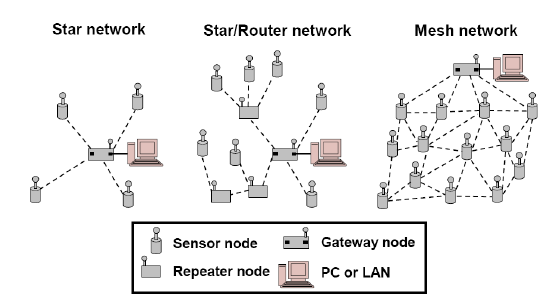
\includegraphics[width=0.65\linewidth]{figuras/topologias.png} 
        \label{fig:topologias}
        \\ \small Fonte: GTA/UFRJ (2018).
    \end{figure}
\end{frame}

\begin{frame}{Roteamento Hierárquico}
    Um algoritmo altamente usado nas RSSFs é o LEACH (\textit{Low-Energy Adaptive Clustering Hierarchy}), aplicado com base na topologia árvore/\textit{cluster}. Usando esse conceito, os nós sensores são segmentados em grupos menores onde cada grupo tem um nó líder ou nó principal, que recebe os dados dos outros sensores e faz a comunicação com a estação-base.
\end{frame}

\begin{frame}{Roteamento Hierárquico (Continuação)}
    Antes da transmissão, o nó líder (também chamado de \textit{cluster-head}) faz um pré-processamento para decidir se haverá agregação dos dados, assim economizando no número de transmissões e gastando menos energia. Este nó também garante o controle de transmissões, permitindo que apenas um nó sensor seja ligado para transmissão por vez.

    
    Neste protocolo, os líderes não são fixos. Na fase de inicialização, cada nó transmite sua energia disponível e sua localização para a estação-base, na qual irá definir os \textit{clusters} e o nó líder, que é escolhido dentre os nós com maior energia restante.
\end{frame}

\begin{frame}{Roteamento Hierárquico (Ilustração)}
    \begin{figure}
        \centering
        \caption{Roteamento Hierárquico}
        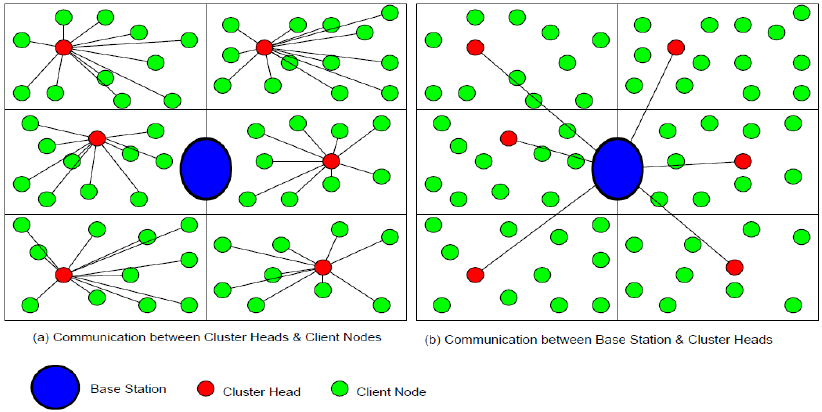
\includegraphics[width=0.7\linewidth]{figuras/roteamento hierarquico.png} 
        \label{fig:roteamento hierarquico}
        \\ \small Fonte: GTA/UFRJ (2018).
    \end{figure}
\end{frame}

\begin{frame}{Roteamento Orientado a Dados}
    Um outro protocolo também usado é o \textit{Directed Diffusion}, no qual seu roteamento se baseia unicamente em dados, não na hierarquia ou em endereços específicos. Nessa abordagem, a comunicação é estabelecida através do nome ou tipo de dado que deseja obter, onde um nó “sorvedouro” (\textit{sink}) solicita uma informação específica denominada “interesse”. Este interesse é difundido (\textit{broadcast}) pela rede até encontrar sensores que contenham tal informação.
\end{frame}

\begin{frame}{Roteamento Orientado a Dados (Continuação)}
    Quando um nó recebe o interesse de um vizinho, ele cria uma rota chamada “gradiente” em seu cache local, que indica a direção para onde os dados correspondentes devem ser enviados (ou seja, para o vizinho interessado). Assim que um sensor detecta o evento ou objeto solicitado, ele começa a enviar os dados seguindo a rota do gradiente estabelecido, podendo até mesmo agregar os dados recebidos pelos outros sensores para fazer um único envio mais completo e economizando no gasto de energia.

    
    Como esses dados podem chegar por diversos caminhos, o nó sorvedouro seleciona um deles (geralmente o que entrega a informação primeiro) e “reforça” o interesse nessa rota, estabelecendo-a como a rota principal para uma coleta de dados mais eficiente. Assim, esse protocolo garante robustez na coleta de dados e economiza energia, visto que evita transmissões desnecessárias das demais rotas. 

\end{frame}

\begin{frame}{Roteamento Orientado a Dados (Ilustração)}
    \begin{figure}
        \centering
        \caption{Roteamento Orientado a Dados}
        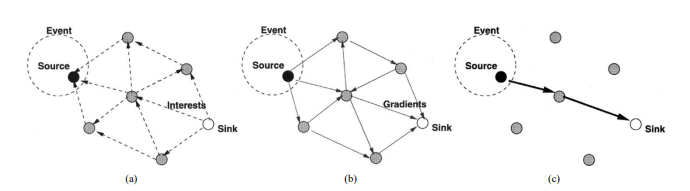
\includegraphics[width=1.0\linewidth]{figuras/roteamento orientado a dados.png} 
        \label{fig:roteamento roteamento orientado a dados}
        \\ \small Fonte: INTANAGONWIWAT; GOVINDAN; ESTRIN (2000).
    \end{figure}
\end{frame}
% \section{Segurança em Ambientes Hostis}
\begin{frame}{Segurança Cibernética em Ambientes Hostis}
    Tendo em vista o funcionamento de uma RSSF, outro aspecto essencial para seu funcionamento é a segurança. Os sensores, ao contrário de outros dispositivos de rede, correm riscos tanto digitais quanto físicos por conta de sua natureza e ambiente.

    \begin{exampleblock}{Exemplo: interferência eletromagnética}
        A exposição de sensores em ambientes veiculares pode causar interferências por conta do motor e outros equipamentos internos que geram ruídos eletromagnéticos, causando queda de desempenho na sensibilidade de transmissão e recepção de dados. O mesmo também cita que sinais de \textit{bluetooth} e Wi-Fi (WLAN) também podem degradar o desempenho dos sensores.
    \end{exampleblock}
\end{frame}

\begin{frame}{Ataques de Identidade}
    Numa RSSF, é praticamente impossível que todos os nós que não se conhecem tenham identidades convincentes. O ataque Sybill, conforme detalhado por Costa, Galetti e Pessanha (2024), consiste em atacar diretamente este ponto fraco da rede, onde um único \textit{hardware} assume múltiplas identidades em uma rede.

    
    Com isso, quando se usa um protocolo LEACH, o atacante consegue manipular sua chance estatística de ser eleito como líder (\textit{cluster-head}) por conta de suas várias identidades. Assim, ele pode criar um monopólio de segurança onde todos os dados de nós confiáveis passem primeiro pelo atacante, interceptando as transmissões.

\end{frame}

\begin{frame}{Ataques de Identidade}
    \begin{figure}
        \centering
        
\includegraphics[width=0.58\linewidth]{figuras/patrick pergunta.PNG} 
        \label{fig:patrick pergunta}
    \end{figure}
\end{frame}

\begin{frame}{Ataques de Identidade}
    \begin{figure}
        \centering
        
\includegraphics[width=0.55\linewidth]{figuras/bob esponja responde.PNG} 
        \label{fig:bob esponja responde}
    \end{figure}
\end{frame}

\begin{frame}{Estratégias de Resiliência}
    Tendo em vista como funcionam esses ataques, é necessário alguns métodos reforçados de segurança. Provavelmente a mais óbvia de se pensar seria o sistema de senhas e criptografia da rede, mas isso pode não ser viável por conta do alto consumo de energia e memória.

\end{frame}

\begin{frame}{Mecanismo de Reputação}
    Alternativamente, podemos usar o Mecanismo de Reputação, onde os nós observam o comportamento de seus vizinhos (como se estão enviando ou alterando pacotes de dados de forma suspeita). Nessa abordagem, cada nó mantém uma pontuação de confiabilidade dos seus vizinhos. Assim, se a reputação de algum vizinho cai abaixo de um limite, ele é simplesmente ignorado pela rede nas rotas de comunicação.

\end{frame}

\begin{frame}{Proteção da Camada Física}
    Entretanto, não é apenas a camada de rede que deve ser protegida, visto que o sinal dos sensores também pode ser alvo de ataque. Para resolver esse problema, a camada física foca em proteger a interceptação ou bloqueio do sinal de rede, adotando a técnica de espalhamento de espectro (FHSS/DSSS), na qual a ideia se baseia em ficar trocando a frequência do sinal. Dessa forma, caso uma frequência seja bloqueada, o sensor consegue trocar para outra.

\end{frame}
% \section{O Futuro: Edge AI}

\begin{frame}{Inteligência Artificial de Borda (Edge AI)}
    \begin{columns}
        % --- COLUNA DA ESQUERDA (TEXTO) ---
        \begin{column}{0.55\textwidth}
            \begin{itemize}
                \item O futuro das RSSF transforma os nós sensores, antes coletores passivos, em unidades de processamento inteligente.  
                \item O \textit{Edge Computing} move a análise para a periferia da rede, eliminando a total dependência da nuvem.  
                \item Isso é viabilizado pelo \textbf{TinyML}, que roda modelos de redes neurais diretamente nos microcontroladores.  
            \end{itemize}
            
            \vspace{0.2cm}
            
            \begin{block}{A Vantagem Energética}
                O nó processa dados localmente e transmite via rádio \textbf{apenas a inferência} (resultado), economizando drasticamente a bateria.  
            \end{block}
        \end{column}
        
        % --- COLUNA DA DIREITA (IMAGEM) ---
        \begin{column}{0.45\textwidth}
            \begin{figure}
                \centering
                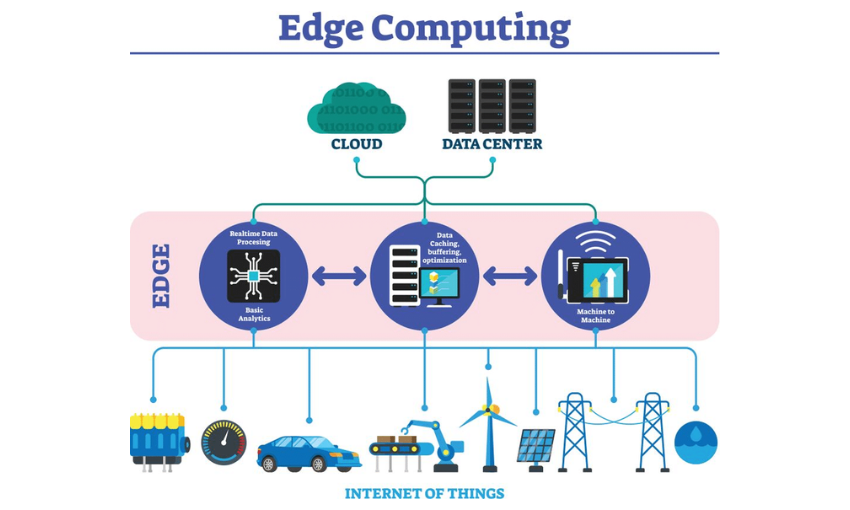
\includegraphics[width=\textwidth]{figuras/edge.png}
                \caption{A camada de Edge Computing.}
                \vspace{0.1cm}
                {\tiny Fonte: Portal Embarcados}
            \end{figure}
        \end{column}
    \end{columns}
\end{frame}

\begin{frame}{Impactos Diretos na Indústria 4.0}
    \begin{columns}
        \begin{column}{0.5\textwidth}
            \begin{itemize}
                \item A integração entre IoT e IA fornece os dados processados necessários para alimentar \textbf{Gêmeos Digitais} (\textit{Digital Twins}).  
                \item As indústrias conseguem simular o comportamento físico de seus equipamentos e prever falhas com precisão cirúrgica.  
                \item Os nós atuam como o sistema nervoso das fábricas, transformando a rede em um sistema de tomada de decisão proativo.  
            \end{itemize}
        \end{column}
        
        \begin{column}{0.5\textwidth}
            \begin{center}
                \textbf{Projeção de Impacto Econômico}\vspace{0.4cm}
                
                % --- INFOGRÁFICO FEITO EM LATEX (TIKZ) ---
                \begin{tikzpicture}
                    % Círculo 1: Manutenção (-40%)
                    \fill[cyan!10] (0,0) circle (1.1);
                    \draw[cyan!80!blue, line width=1mm] (0,0) circle (1.1);
                    \node[cyan!80!black, font=\Large\bfseries] at (0,0) {-40\%};
                    \node[align=center, font=\footnotesize] at (0,-1.6) {Custos de\\Manutenção};
                    
                    % Círculo 2: Downtime (-50%)
                    \fill[orange!10] (3,0) circle (1.1);
                    \draw[orange!80!red, line width=1mm] (3,0) circle (1.1);
                    \node[orange!80!black, font=\Large\bfseries] at (3,0) {-50\%};
                    \node[align=center, font=\footnotesize] at (3,-1.6) {Tempo de\\Parada};
                \end{tikzpicture}
                
                \vspace{0.6cm}
                {\tiny \textit{Fonte: McKinsey \& Company (Digital Manufacturing)}}
            \end{center}
        \end{column}
    \end{columns}
\end{frame}
% \section{Conclusão}

\begin{frame}{Síntese dos Desafios e Soluções}
    \begin{itemize}
        \item As RSSF representam o pilar fundamental para a Internet das Coisas (IoT) e para a Indústria 4.0, superando as limitações físicas dos cabeamentos.  
        \item O maior gargalo técnico é a gestão energética: a sobrevivência de toda a malha depende da eficiência individual de cada sensor.  
        \item Nas camadas inferiores, protocolos de ciclo de trabalho (como o T-MAC) provaram ser indispensáveis para mitigar o desperdício crítico da escuta ociosa.  
        \item No roteamento, a transição para arquiteturas de múltiplos saltos (\textit{multi-hop}) e agregação de dados descentraliza a carga e estende a cobertura.
        \item A integridade do sistema é garantida por protocolos  
    \end{itemize}
\end{frame}

\begin{frame}{Considerações Finais}
    \begin{itemize}
        \item As redes evoluíram de sistemas dependentes de estações-base centralizadoras para organismos distribuídos.  
        \item O uso do aprendizado de máquina na borda (Edge AI) resolve o problema do desgaste da bateria evitando transmissões pesadas.  
    \end{itemize}

    \vspace{0.5cm}

    \begin{block}{O Caminho Definitivo}
        A integração entre a microeletrônica de baixíssimo consumo e a Inteligência Artificial de borda é o caminho consolidado para sistemas de monitoramento autônomos e economicamente viáveis.  
    \end{block}
    
    \vspace{0.5cm}
    

\end{frame}

% ==========================================

% exemplos

%==========================================

\section{Introdução} % O comando \section é o que cria a bolinha no topo
\begin{frame}{Início do Trabalho}
    teste com bolinha no topo
    
    em baixo no rodapé tem nosso nomee, titulo e ano
\end{frame}

\section{Camada Física} 
\begin{frame}{Exemplos de Blocos}
    \begin{block}{Definição Técnica}
        Texto padrão para conceitos e fundamentos das RSSF.
    \end{block}

    \begin{exampleblock}{Exemplo Prático (Página 3)}
        Este é o bloco verde para exemplos. Caso a gente queira adicionar mais blocos estilizados é só por. Mas por enquanto coloquei só esses dois.
    \end{exampleblock}
\end{frame}

\end{document}
